\subsection{Суммарные затраты на реализацию программного проекта} \label{sum_cost}

Круговая диаграмма, отображающая структуру затрат проекта,  приведена на рисунке \ref{img:sum_cost}. Расчёт суммарных затрат на реализацию программного проекта приведён в таблице \ref{table:sum_cost}.

\begin{table} [h!]
  \captionsetup{justification=raggedright}
  \caption{Суммарные затраты на проект}\label{table:sum_cost}
 \begin{center}
  \begin{tabular}{| c | >{\centering}m{8cm} | >{\centering}m{4cm} |}
  \hline
 \rowcolor{Gray} №  & Статья расходов & Затраты, руб. \tabularnewline \hline

 1 & Заработная плата исполнителям $C_\textrm{ЗАРП}$ & 338 966,54 \tabularnewline \hline
 2 & Закупка и аренда оборудования $C_\textrm{ОБ}$ & 22 533 \tabularnewline \hline
 3 & Организация рабочих мест $C_\textrm{ОРГ}$ & 54 000 \tabularnewline \hline
 4 & Накладные расходы $C_\textrm{НАКЛ}$ & 130 371,75 \tabularnewline \hline
 \multicolumn{2}{|l|}{Суммарные затраты} & 545 871,29 \tabularnewline \hline

   \end{tabular}
 \end{center}
\end{table}

\begin{figure} [h!] 
  \center
  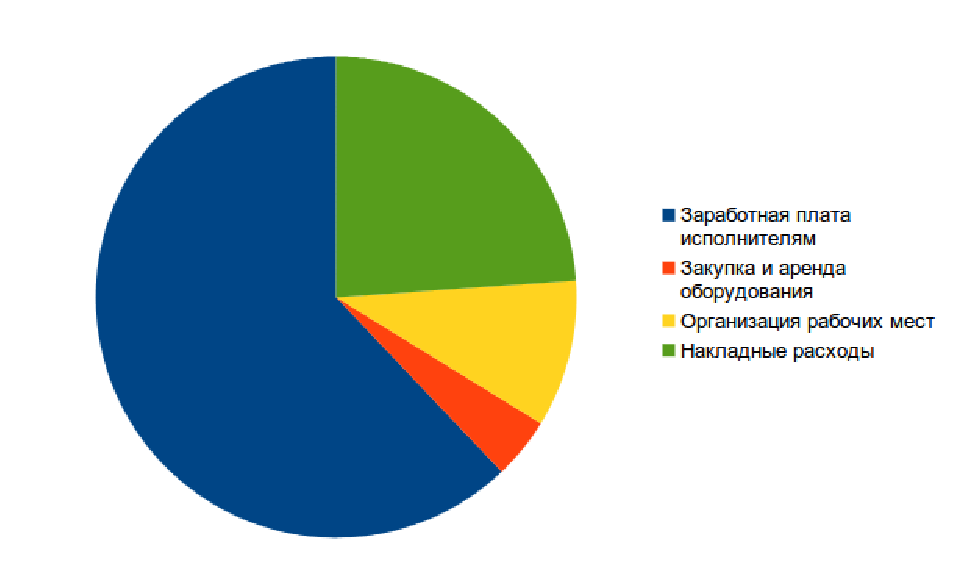
\includegraphics [scale=1] {sum_cost}
  \caption{Структура затрат проекта} 
  \label{img:sum_cost}  
\end{figure}
\FloatBarrier